% #######################################
% ########### FILL THESE IN #############
% #######################################
\def\mytitle{LINE ASSIGNMENT}
\def\mykeywords{}
\def\myauthor{SIVA PARVATHI TUNGALA}
\def\contact{tvssn143@gmail.com}
\def\mymodule{ Future Wireless Communication(FWC22089)}
% #######################################
% #### YOU DON'T NEED TO TOUCH BELOW ####
% #######################################
\newcommand{\myvec}[1]{\ensuremath{\begin{pmatrix}#1\end{pmatrix}}}
\let\vec\mathbf
\providecommand{\pr}[1]{\ensuremath{\Pr\left(#1\right)}}
\providecommand{\qfunc}[1]{\ensuremath{Q\left(#1\right)}}
\providecommand{\sbrak}[1]{\ensuremath{{}\left[#1\right]}}
\providecommand{\lsbrak}[1]{\ensuremath{{}\left[#1\right.}}
\providecommand{\rsbrak}[1]{\ensuremath{{}\left.#1\right]}}
\providecommand{\brak}[1]{\ensuremath{\left(#1\right)}}
\providecommand{\lbrak}[1]{\ensuremath{\left(#1\right.}}
\providecommand{\rbrak}[1]{\ensuremath{\left.#1\right)}}
\providecommand{\cbrak}[1]{\ensuremath{\left\{#1\right\}}}
\providecommand{\lcbrak}[1]{\ensuremath{\left\{#1\right.}}
\providecommand{\rcbrak}[1]{\ensuremath{\left.#1\right\}}}
\documentclass[10pt, a4paper]{article}
\usepackage[a4paper,outer=1.5cm,inner=1.5cm,top=1.75cm,bottom=1.5cm]{geometry}
\twocolumn
\usepackage{circuitikz}
\usepackage{amsmath,bm}
\usepackage{amsthm}
\usepackage{mathtools}
\usepackage{amsfonts}
\usepackage{amssymb}
\usepackage{graphicx}
\usepackage{bm}
\newcommand{\bfitDelta}{\bm{\mathit{\Delta}}}

\graphicspath{{./images/}}
%colour our links, remove weird boxes
\usepackage[colorlinks,linkcolor={black},citecolor={blue!80!black},urlcolor={blue!80!black}]{hyperref}
%Stop indentation on new paragraphs
\usepackage[parfill]{parskip}
%% Arial-like font
\usepackage{lmodern}
\renewcommand*\familydefault{\sfdefault}
%Napier logo top right
\usepackage{watermark}
%Lorem Ipusm dolor please don't leave any in you final report ;)
\usepackage{karnaugh-map} 
\usepackage{tabularx}
\usepackage{lipsum}
\usepackage{xcolor}
\usepackage{listings}
%give us the Capital H that we all know and love
\usepackage{float}
%tone down the line spacing after section titles
\usepackage{titlesec}
%Cool maths printing
\usepackage{amsmath}
%PseudoCode
\usepackage{algorithm2e}

\titlespacing{\subsection}{0pt}{\parskip}{-3pt}
\titlespacing{\subsubsection}{0pt}{\parskip}{-\parskip}
\titlespacing{\paragraph}{0pt}{\parskip}{\parskip}
\newcommand{\figuremacro}[5]{
    \begin{figure}[#1]
        \centering
        \includegraphics[width=#5\columnwidth]{#2}
        \caption[#3]{\textbf{#3}#4}
        \label{fig:#2}
    \end{figure}
}


 \lstset{
frame=single, 
breaklines=true,
columns=fullflexible
}
\thiswatermark{\centering \put(1,-110){
\includegraphics[scale=0.05]{iitlogo.jpg}} }
\title{\mytitle}
\author{\myauthor\hspace{1em}\\\contact\\IITH\hspace{0.5em}-\hspace{0.5em}\mymodule}
\date{}
\hypersetup{pdfauthor=\myauthor,pdftitle=\mytitle,pdfkeywords=\mykeywords}
\sloppy
% #######################################
% ########### START FROM HERE ###########
% #######################################
\begin{document}
 \maketitle
 \tableofcontents
 
 \Large\section{Problem}
 Q.Straight lines 3x+4y=5 and 4x-3y=15 intersect at point A. Points B and C are choosen on these two lines such that AB=AC. Determine the possible equations of the line BC through the point (1,2).
 
 \section{Solution}
we know that vector equation of the lines intersecting at point A, 
\begin{align}
 \textbf{n}_{1}^{\top}\textbf{A}=c_1 \\
  \textbf{n}_{2}^{\top}\textbf{A}=c_2
\end{align}
The vector equation of the line1 and line2 are
\begin{align}
  \textbf{n}_{1}^{\top}\textbf{B}=c_1 \\
  \textbf{n}_{2}^{\top}\textbf{C}=c_2
\end{align}
\centering
\begin{tabular}{|c |c |}
     \hline % <-- Alignments: 1st column left, 2nd middle and 3rd right, with vertical lines in between
	\large\textbf{Symbol} & \large\textbf{Co-ordinates}  \\
       \hline
	\large \textbf{n1} & $\ \begin{pmatrix} 3\\ 4 \end{pmatrix}$  \\
        \hline
	\large \textbf{n2} & $\ \begin{pmatrix} 4\\ -3 \end{pmatrix}$  \\
        \hline
	 \large \textbf{R} & $\ \begin{pmatrix}0 & 1 \\ -1 & 0 \end{pmatrix}$ \\
       \hline
     \large \textbf{p} & $\ \begin{pmatrix} 1\\ 2 \end{pmatrix}$  \\
        \hline
    \end{tabular}
\\
from equation (1) and (2), \\
$ \textbf{A} =\myvec{\textbf{n}_{1}^{\top} \\ \textbf{n}_{2}^{\top}}^{-1}\myvec{{c}_{1} \\ {c}_{2}}$\\
$\textbf{A}=\myvec{3\\ -1} $\\ 
Points B and C are choosen on these two lines such that AB = AC i.e.,
\begin{align}
\| \textbf{A-B} \| = \| \textbf{A-C} \| 
\end{align}
\raggedright Consider, \\
\begin{align}
\textbf{B} = \textbf{A}+{K}_{1}\textbf{m}_{1}\\
\textbf{C} = \textbf{A}+{K}_{2}\textbf{m}_{2}
\end{align}
when a line passing through a point the vector equation is,
\begin{align}
\textbf{n}^{\top}(\textbf{x}-\textbf{p})=0 \\
where ,  \textbf{n}=\textbf{R}(\textbf{B}-\textbf{C})
\end{align}
\raggedright Substituting B and C in eq(5), \\
$\hspace*{2.5cm}|{K}_{1}|\|\textbf{m}_{1}\|=|{K}_{2}|\|\textbf{m}_{2}\| $\\
\begin{align}
if \hspace*{0.1cm}\|\textbf{m}_{1}\| = \|\textbf{m}_{2}\| = 1 \\
then , {K}_{1}={K}_{2} (or){K}_{1}=-{K}_{1}\\
\end{align}
To satisfy equation(10),\\
\begin{align}
\textbf{m}_{1}=\frac{\textbf{R}\textbf{n}_{1}}{\|\textbf{n}_{1}\|} \\
\textbf{m}_{2}=\frac{\textbf{R}\textbf{n}_{2}}{\|\textbf{n}_{2}\|} 
\end{align}
\raggedright let $ {K}_{1} $\hspace*{0.1cm}be $ \lambda $ \hspace*{0.1cm} then , \\
\raggedright Case(i) : \\
\begin{align}
\textbf{B} = \textbf{A}+\lambda\textbf{m}_{1}\\
\textbf{C} = \textbf{A}+\lambda\textbf{m}_{2}
\end{align}
Substitute B and C in eq(9),\\
\begin{align}
\textbf{n}=\lambda\textbf{R}^{2}(\frac{\textbf{n}_{1}}{\| \textbf{n}_{1} \|}-\frac{\textbf{n}_{2}}{\| \textbf{n}_{2} \|}) \\
\textbf{n}=-\lambda(\frac{\textbf{n}_{1}}{\| \textbf{n}_{1} \|}-\frac{\textbf{n}_{2}}{\| \textbf{n}_{2} \|})
\end{align}
As eq(8) is satisfied by B, substitute n and B in (8) \\
\begin{align}
-\lambda(\frac{\textbf{n}_{1}}{\| \textbf{n}_{1} \|}-\frac{\textbf{n}_{2}}{\| \textbf{n}_{2} \|})^\top(\textbf{A}-\textbf{p}+\lambda\textbf{m}_{1})=0 \\
\lambda=\frac{(\frac{\textbf{n}_{1}}{\| \textbf{n}_{1} \|}-\frac{\textbf{n}_{2}}{\| \textbf{n}_{2} \|})^\top(\textbf{A}-\textbf{p})}{\frac{\textbf{n}_{2}^\top\textbf{m}_{1}}{\| \textbf{n}_{2} \|}}\\
\lambda=\frac{(\| \textbf{n}_{2} \|\textbf{n}_{1}-\| \textbf{n}_{1} \|\textbf{n}_{2})^\top(\textbf{A}-\textbf{p})}{\textbf{n}_{2}^\top\textbf{n}_{1}\textbf{R}}
\end{align}
\raggedright Similarly, Case(ii) : \\
\begin{align}
\textbf{B} = \textbf{A}+\lambda\textbf{m}_{1}\\
\textbf{C} = \textbf{A}-\lambda\textbf{m}_{2}
\end{align}
Substitute B and C in eq(9),\\
\begin{align}
\textbf{n}=-\lambda(\frac{\textbf{n}_{1}}{\| \textbf{n}_{1} \|}+\frac{\textbf{n}_{2}}{\| \textbf{n}_{2} \|})\\
\lambda=-\frac{(\| \textbf{n}_{2} \|\textbf{n}_{1}-\| \textbf{n}_{1} \|\textbf{n}_{2})^\top(\textbf{A}-\textbf{p})}{\textbf{n}_{2}^\top\textbf{n}_{1}\textbf{R}}
\end{align}
By sustituting in eq(19) and (23),
\begin{align}
\lambda=\myvec{230 \\ 110}
\end{align}
from Case(i), by substituting the values \\
\begin{align}
\textbf{B}=\myvec{-181 \\ 137} and\hspace{0.3cm}\textbf{C}=\myvec{141 \\ 183} \\
\textbf{n}=\myvec{46\\ 183}
\end{align}
from Case(ii), by substituting the values \\
\begin{align}
\textbf{B}=\myvec{-85 \\ 65} and \hspace{0.3cm}\textbf{C}=\myvec{63 \\ -89} \\
\textbf{n}=\myvec{-154\\ -22} 
\end{align}
%  Therefore,the possible equations passing through the point(1,2) are 7y-x-13=0 and 7x+y-9=0.\\
%   \section{Plot}
%\begin{figure}
%       \centering
%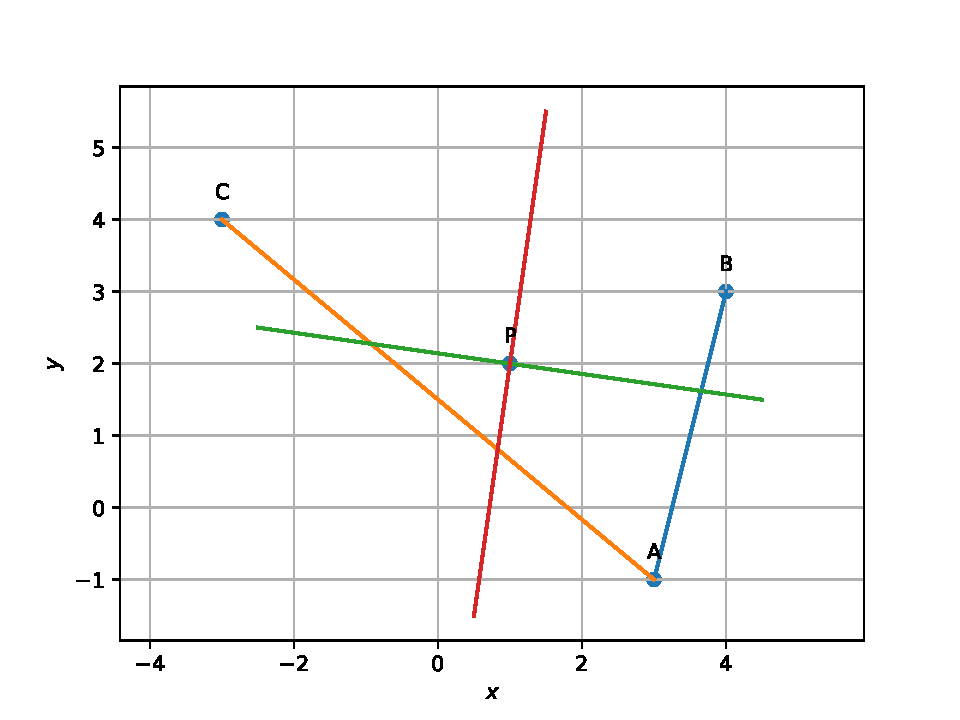
\includegraphics[width=\columnwidth]{fig.pdf}
%       \label{fig:my_label}
%\end{figure}
        Therefore,the possible equations passing through the point(1,2) are 7y-x-13=0 and 7x+y-9=0.\\
   \section{Plot}
\begin{figure}
       \centering
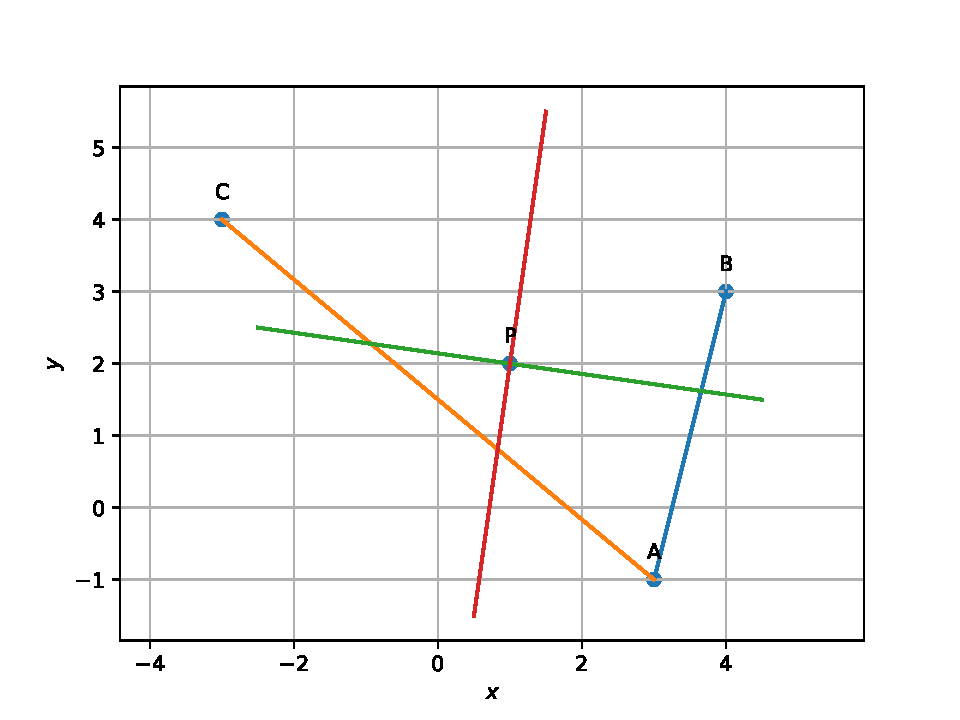
\includegraphics[width=\columnwidth]{fig.pdf}
       \label{fig:my_label}
\end{figure}

\section{Software}
  We can get the parallel equation of given equation and the plot of two equtions by executing the following code:
 \vspace{1mm} 
\begin{lstlisting}
https://github.com/sivaparvathi-tungala/fwc_module_1/tree/main/line
\end{lstlisting}
\end{document}\